\documentclass[a4paper,12pt,twoside]{../includes/ThesisStyle}
\usepackage[utf8]{inputenc}
\usepackage[T1]{fontenc}

\usepackage[left=1.5in,right=1.3in,top=1.1in,bottom=1.1in,includefoot,includehead,headheight=13.6pt]{geometry}\renewcommand{\baselinestretch}{1.05}


% =============================================================================
%\usepackage[sectionbib]{chapterbib}	% Cross-reference package (Natural BiB)
%\usepackage{bibunits}
%\usepackage{natbib}					% Put References at the end of each chapter
\usepackage{algorithm}
\usepackage{alltt}
\usepackage{amsfonts}
\usepackage{amsmath}
\usepackage{amssymb}
\usepackage{cite}
\usepackage{color}
\usepackage{enumerate}
\usepackage{booktabs} % used for \midrule
\usepackage{fancyhdr}					% Fancy Header and Footer
\usepackage{graphicx}
\usepackage{ifthen}
\usepackage{latexsym}
\usepackage{multirow}
\usepackage{rotating}					% Sideways of figures & tables
\usepackage{stmaryrd}
\usepackage{subfigure}
\usepackage{url}         
\usepackage{xspace}
\usepackage[normalem]{ulem} % for \sout
\usepackage{xcolor}
\usepackage{tablefootnote}
\usepackage{pifont}

% =============================================================================

% Table of contents for each chapter
\usepackage[nottoc, notlof, notlot]{tocbibind}
\usepackage{minitoc}
\setcounter{minitocdepth}{1}
\mtcindent=15pt

\setcounter{secnumdepth}{3}
\setcounter{tocdepth}{2}
  
% =============================================================================
% Fancy Header Style Options

\pagestyle{fancy}                       % Sets fancy header and footer
\fancyfoot{}                            % Delete current footer settings

%\renewcommand{\chaptermark}[1]{         % Lower Case Chapter marker style
%  \markboth{\chaptername\ \thechapter.\ #1}}{}} %

%\renewcommand{\sectionmark}[1]{         % Lower case Section marker style
%  \markright{\thesection.\ #1}}         %

\fancyhead[LE,RO]{\bfseries\thepage}    % Page number (boldface) in left on even
% pages and right on odd pages
\fancyhead[RE]{\bfseries\nouppercase{\leftmark}}      % Chapter in the right on even pages
\fancyhead[LO]{\bfseries\nouppercase{\rightmark}}     % Section in the left on odd pages

\let\headruleORIG\headrule
\renewcommand{\headrule}{\color{black} \headruleORIG}
\renewcommand{\headrulewidth}{1.0pt}
\usepackage{colortbl}
\arrayrulecolor{black}

\fancypagestyle{plain}{
  \fancyhead{}
  \fancyfoot{}
  \renewcommand{\headrulewidth}{0pt}
}


% =============================================================================
% Clear Header Style on the Last Empty Odd pages
\makeatletter

\def\cleardoublepage{\clearpage\if@twoside \ifodd\c@page\else%
  \hbox{}%
  \thispagestyle{empty}%              % Empty header styles
  \newpage%
  \if@twocolumn\hbox{}\newpage\fi\fi\fi}

\makeatother

\newenvironment{maxime}[1]
{
\vspace*{0cm}
\hfill
\begin{minipage}{0.5\textwidth}%
%\rule[0.5ex]{\textwidth}{0.1mm}\\%
\hrulefill $\:$ {\bf #1}\\
%\vspace*{-0.25cm}
\it 
}%
{%

\hrulefill
\vspace*{0.5cm}%
\end{minipage}
}

\let\minitocORIG\minitoc
\renewcommand{\minitoc}{\minitocORIG \vspace{1.5em}}


\renewcommand{\epsilon}{\varepsilon}

% centered page environment
\newenvironment{vcenterpage}
	{\newpage\vspace*{\fill}\thispagestyle{empty}\renewcommand{\headrulewidth}{0pt}}
	{\vspace*{\fill}}
	

%=============================================================================

\usepackage{needspace}
\newcommand{\needlines}[1]{\Needspace{#1\baselineskip}}

\usepackage{xcolor}
\definecolor{source}{gray}{0.95}
% source code formatting
\usepackage{listings}
    % global settings for source code listing package
\lstset{
    basicstyle=\ttfamily\small,
    showspaces=false,
    showstringspaces=false,
    captionpos=b, 
    columns=fullflexible}

\lstdefinelanguage{ST}{
    keywordsprefix=\#,
    morekeywords=[0]{true,false,nil},
    morekeywords=[1]{self,super,thisContext},
    morekeywords=[2]{ifTrue:,ifFalse:,whileTrue:,whileFalse:,and:,or:,xor:,not:,by:,timesRepeat:},
    sensitive=true,
    morecomment=[s]{"}{"},
    morestring=[d]',
    escapechar={!},
    alsoletter={., :, -, =, +, <},
    moredelim=**[is][\itshape]{/+}{+/},
    literate=
        {^}{{$\uparrow$}}1
        {:=}{{$\leftarrow$}}1
        {~}{{$\sim$}}1
        {-}{{\sf -\hspace{-0.13em}-}}1  % the goal is to make - the same width as +
        {+}{\raisebox{0.08ex}{+}}1		% and to raise + off the baseline to match V
        , % Don't forget the comma at the end!
    style=STStyle
}
\lstdefinestyle{STStyle}{
    tabsize=4,
    %frame=leftline,
    % frame=bl,
    %framerule=2pt,
    %rulecolor=\color{gray},
    % backgroundcolor=\color{white},
    %backgroundcolor=\usebeamercolor[bg]{listing},
    basicstyle=\ttfamily\small,
    keywordstyle=\bf\ttfamily,
    % stringstyle=\color{orange},
    stringstyle=\mdseries\slshape,
    commentstyle=\it\rmfamily\color{darkgray}, 
    commentstyle=\mdseries\slshape\color{gray},
    %commentstyle=\mdseries\slshape,
    emphstyle=\bf\ttfamily,
    escapeinside={!}{!},
	%backgroundcolor=\color{source},
    %emphstyle={[2]\color{red}},
    %emphstyle={[3]\color{blue}\bf},
    %emphstyle={[4]\color{blue}},
    keepspaces=true
} 

%\lstnewenvironment{javacode}  [1][]{\lstset{language=java,#1}\needlines{#2}}{} 
%\lstnewenvironment{pythoncode}[2][]{\lstset{language=python,#1}\needlines{#2}}{}
\lstnewenvironment{stcode}    [2][]{\lstset{language=ST,#1}\needlines{#2}}{}
\lstnewenvironment{ccode}     [2][]
    {\lstset{language=C,numbers=left,escapechar=\$,numberstyle=\tiny,#1}\needlines{#2}}{}

% ON: I tried to pass the line number options in as arg #1 but it does not work for me
% I also could net get the line numbers to consistently increase
\lstnewenvironment{numstcode} [2][]
    {\lstset{language=ST,numbers=left,numberstyle=\tiny,numbersep=2pt,#1}\needlines{#2}}{}
\lstnewenvironment{numstcodecont} [2][]
    {\lstset{language=ST,numbers=left,numberstyle=\tiny,numbersep=2pt,firstnumber=last#1}\needlines{#2}}{}

\newcommand{\lst}[1]{{\tt #1}}

% In-line code (literal)

% In-line code (latex enabled)
% Use this only in special situations where \ct does not work
% (within Section headings ...):
\newcommand{\lct}[1]{{\textsf{\textup{#1}}}}
% Code environments
\lstnewenvironment{code}{%
	\lstset{%
		% frame=lines,
		frame=single,
		framerule=0pt,
		mathescape=false
	}
}{}

%\renewcommand{\lstlistingname}{Code Example}

% =============================================================================
\newboolean{showcomments}
\setboolean{showcomments}{true}

\ifthenelse{\boolean{showcomments}} {
	\newcommand{\ugh}[1] {\textcolor{red}{\uwave{#1}}}	% please rephrase
	\newcommand{\ins}[1] {\textcolor{blue}{\uline{#1}}}	% please insert
	\newcommand{\del}[1] {\textcolor{red}{\sout{#1}}}	% please delete
	\newcommand{\chg}[2] {								% please change
		\textcolor{red}{\sout{#1}}{\ra}
		\textcolor{blue}{\uline{#2}}}
	\newcommand{\nbc}[3]{								% comment
		{\colorbox{#3}{\bfseries\sffamily\scriptsize\textcolor{white}{#1}}}
		{\textcolor{#3}{\sf\small$\blacktriangleright$\textit{#2}$\blacktriangleleft$}}}

}{
	\newcommand{\ugh}[1]{#1}							% please rephrase
	\newcommand{\ins}[1]{#1}							% please insert
	\newcommand{\del}[1]{}								% please delete
	\newcommand{\chg}[2]{#2}							% please change
	\newcommand{\nbc}[3]{}								% comment
}

% =============================================================================
\usepackage[pagebackref,hyperindex=true]{hyperref}


% Links in pdf
\usepackage{color}
\definecolor{linkcol}{rgb}{0.0, 0.0, 0.0} 
\definecolor{citecol}{rgb}{0.0, 0.0, 0.0} 

% Change this to change the informations included in the pdf file
% See hyperref documentation for information on those parameters
\hypersetup {
	bookmarksopen=true,
	pdftitle="Design and Use of Anatomical Atlases for Radiotherapy",
	pdfauthor="Olivier COMMOWICK", 
	pdfsubject="Creation of atlases and atlas based segmentation", %subject of the document
	%pdftoolbar=false, % toolbar hidden
	pdfmenubar=true, %menubar shown
	pdfhighlight=/O, %effect of clicking on a link
	colorlinks=true,
	pdfpagemode=UseNone,
	pdfpagelayout=SinglePage,
	pdffitwindow=true,
	linkcolor=linkcol,
	citecolor=citecol,
	urlcolor=linkcol
}

% =============================================================================
\newcommand{\figlabel}[1] {\label{fig:#1}}
\newcommand{\chaplabel}[1]{\label{chap:#1}}
\newcommand{\seclabel}[1] {\label{sec:#1}}
\newcommand{\tablabel}[1] {\label{tab:#1}}
\newcommand{\lstlabel}[1] {\label{lst:#1}}

\newcommand{\figref}[1] {Figure~\ref{fig:#1}}
\newcommand{\chapref}[1]{Chapter~\ref{sec:#1}}
\newcommand{\secref}[1] {Section~\ref{sec:#1}}
\newcommand{\tabref}[1] {Table~\ref{tab:#1}}
\newcommand{\lstref}[1] {Listing~\ref{tab:#1}}

\newcommand{\commented}[1]{}

\newcommand{\bs}    {\symbol{'134}} % backslash
\newcommand{\us}    {\symbol{'137}} % underscore
\newcommand{\ttt}[1]{\texttt{#1}}
\newcommand{\ie}    {\emph{i.e.},\xspace}
\newcommand{\eg}    {\emph{e.g.},\xspace}
\newcommand{\etal}  {\emph{et al.}\xspace}
\newcommand{\ns}    {\!\!\!\!} %big negative space
\newcommand{\cnull} {\textbackslash0\xspace}


\newcommand\fix[1]{\nb{FIX}{#1}}
\newcommand\todo[1]{\nb{TO DO}{#1}}
\newcommand\cb[1]{\nbc{CB}{#1}{purple}}
\newcommand\sd[1]{\nbc{SD}{#1}{orange}}
\newcommand\is[1]{\nbc{IS}{#1}{gray}}
\newcommand\gc[1]{\nbc{GC}{#1}{olive}}
\newcommand\ct[1]{\nbc{CT}{#1}{teal}}
\newcommand\md[1]{\nbc{MD}{#1}{blue}}
\newcommand\dc[1]{\nbc{DC}{#1}{green}}

% =============================================================================
\newcommand{\NBFFI}  {Native\-Boost-FFI\xspace}
\newcommand{\NB}  {Native\-Boost\xspace}
\newcommand{\B}   {Benzo\xspace}
\newcommand{\ST}  {Small\-talk\xspace}
\newcommand{\PH}  {Pharo\xspace}
\graphicspath{{.}{../figures/}}

\begin{document}
% ===========================================================================

\chapter{\B Prototype Validation}
\chaplabel{validation}
\minitoc
% ===========================================================================
\introduction
% ===========================================================================

In \chapref{ffi} we presented \NB, a mature language-side \FFI implementation that makes heavy use of \B's infrastructure.
\NB is only one of three applications that are based on \B that were initially outlined in \secref{benzo-usecase}.
While \NB is considered stable, the two other applications are currently only prototypes: dynamic primitives and a language-side \JIT.
Hence we will present the two solutions combined in this chapter.

As first we will present \WF, dynamic primitives based on \B.
\WF takes advantage of the metacircular approach of \PH's \VM and makes the primitive definition available at runtime.
This is a step forward from the typical metacircular approach where the whole reflective power of the host environment can only be used at compile-time.
Once the \VM is compiled, all the high-level definitions that existed at compilation time are no longer accessible from language-side.
\WF tries to make a fraction of the original compile-time definitions accessible.

The second prototype, \NB a language-side \JIT compiler takes the core idea of \WF even further.
\WF is capable of defining new primitives at runtime which are not reentrant: it is not possible to activate \PH methods from within primitives.
However, this is what happens in jitted methods: it is possible to switch seamlessly between native methods and standard \PH methods using bytecode evaluation.
Much like the primitives, the \JIT can not be changed from language-side and this is where we bring \NBJ into play.
\NBJ reimplements the \VM-level \JIT compiler at language-side and uses \B to install the native code.


% ===========================================================================
\newpage
\section{\WF: Dynamic Primitives}
\seclabel{val-waterfall}
% ===========================================================================

\begin{figure}[h]
	\centering
	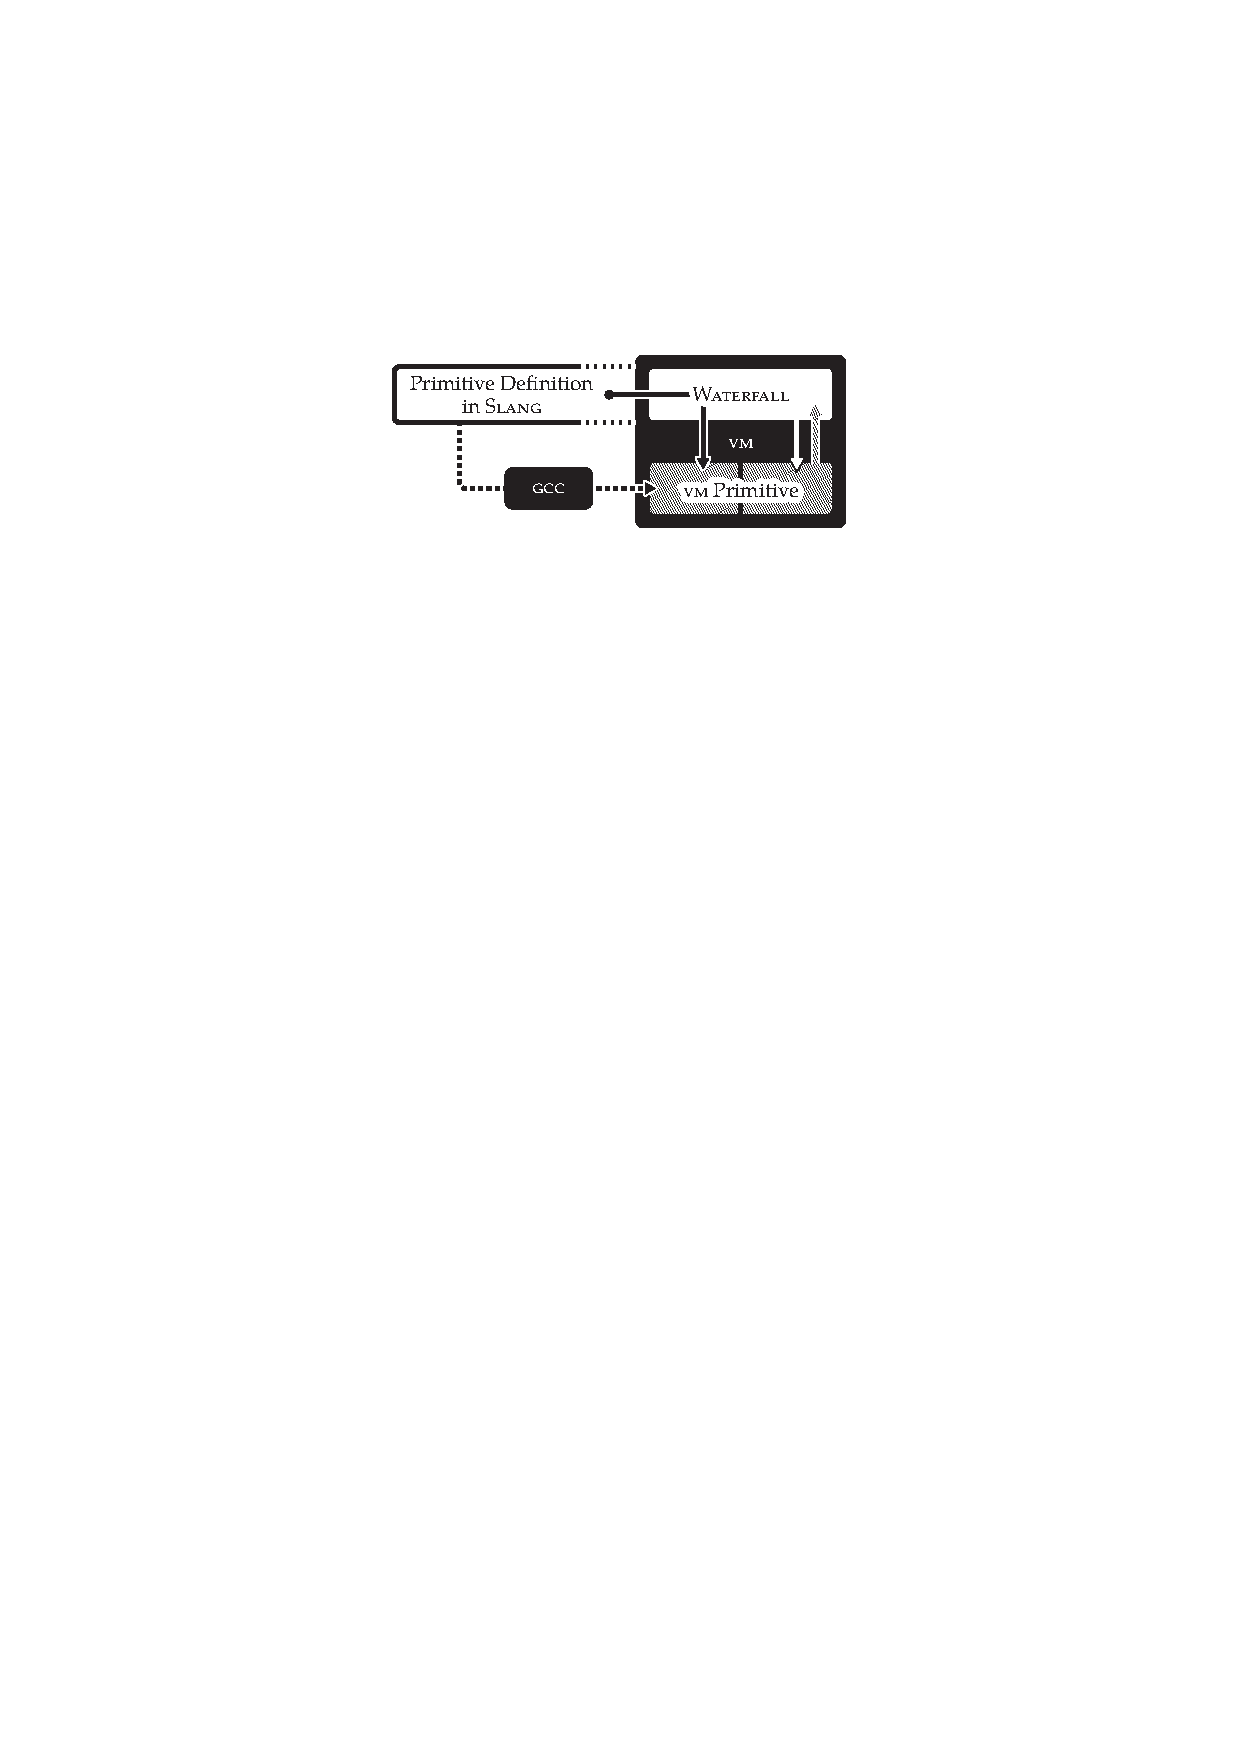
\includegraphics[scale=1.1]{waterfall-overview}
\end{figure}

\noindent In this section we present \WF, a compiler toolchain that allows primitives to be changed dynamically from language-side.
We successfully use \WF to change and recompile whole \VM plugins such as the file plugin as we show in the following \secref{val-waterfall-plugins}.

\WF uses the \B infrastructure to activate native code at runtime.
However, unlike the previously presented \FFI library \WF is not based on directly writing assembler instructions.


% -----------------------------------------------------------------------------
\subsection{Background}
\seclabel{val-waterfall-background}
% -----------------------------------------------------------------------------

The \PH \VM (\urlfootnote{\textsc{Cog}}{http://www.mirandabanda.org/cogblog/}) is developed in a language that is a subset of \ST, known as \Slang, which is transformed to C and then compiled using a standard C compiler.  
\Slang basically has the same syntax as \ST but is semantically constrained to expressions that can be resolved statically at compilation or code generation time and are compatible with C.
Hence \Slang's semantics are closer to C than to \ST. 

The primitives of the \VM are written in \Slang and that is why even in a highly reflective languages such as \ST, where almost every aspect of the language is available for inspection and modification \cite{Denk10a}, primitives can not be changed at runtime.
They can only be intercepted with reflective techniques with considerable performance overheads.
This is an important limitation since primitives are, in general, performance demanding components.
\WF~\cite{Char13a} is a tool that allows developers to change the code written in \Slang for primitives and translate it to native code at runtime.
This replaces the indirection via C that is used in the default compilation process.
Given that \Slang source code can be modified at runtime as any other \ST method, \WF fosters primitives to be dynamically adapted without imposing the common pure reflective techniques performance degradation.

From a high-level point of view \WF provides two services which work transparently: 

\begin{enumerate}
	\item Compilation of \Slang code on demand (lazily).
	\item A clear interface for executing, at runtime and from language-side, the native code generated.
\end{enumerate}

\noindent The first item allows to change the code of primitives at language-side and generate the corresponding native code when needed. 
It also provides the possibility to write methods or functionality with the same \ST syntax but with a static semantic. 
It consists essentially of a transformation toolchain that uses the AST that is generated by the standard \PH compiler harnessing that \Slang and \ST have the same syntax. 
Then this AST representation is translated to native code enforcing C-like \Slang semantics. The current prototype has only three fully implemented stages: \Slang to AST, AST to an IR (between TAC and SSA) and finally AST or IR to native.
The design is open for future additions at any level.
One typical enhancement missing is having different levels of intermediate representations with various techniques on code optimization and register allocation strategies as modern compilers propose \cite[Ch.\ 1]{Appe98a}. 
The second item enables the execution of the dynamically generated native code.
This includes for instance the finding of addresses of \VM internal symbols and all the effort to link the two worlds, \ST and native.
\WF relies on \B for most of this low-level functionality.
In particular \NB, the \B-based \FFI presented in \chapref{ffi}, is used for interfacing with C libraries (\ttt{dlsym}). 

\paragraph{Primitives in \ST}
As already partially explained, whenever a method is compiled with the \ttt{primitive} pragma as shown in \secref{benzo-vm-interaction} a flag is set on the \ttt{CompiledMethod}. 
If the \VM tries to activate such a method, instead of interpreting the bytecodes it calls the corresponding function at \VM-level~\cite{Gold83a}.
%The binding between primitives and numbers is described in a table indexed by number.
\ST distinguishes two types of primitives: essential and non-essential primitives.
Essential primitives are required for the bootstrapping and the essential operations of the language, such as creating a new object or activating a block.
The second category of primitives are mainly used for optimization purposes.

\paragraph{Dynamically Interchangeable Primitives}
\WF uses \B's mechanism for replacing primitive methods with customized versions that are nativized dynamically as described in \chapref{benzo}.
The loophole described there is exploited by \WF to enable dynamic modification of \VM behavior and hence bring primitives to life at language-side.


%----------------------------------------------------------------------------
\paragraph{Benefits} 
We identified two main benefits of changing \VM primitives at runtime:

\begin{enumerate}
	\item Reducing \VM complexity by implementing non-essential primitives reflectively at language-side.
	\item Dynamic instrumentation of primitives.
\end{enumerate}

\paragraph{Reducing \VM Complexity}
\VM extensions are only justified in the presence of strong performance requirements (see \secref{benzo-related}).
All non-essential primitives fall into this category.
Using \WF, these primitives can be implemented at language-side.
This means that these primitives become first-class citizens of the high-level environment and thus evolve with less effort.

\paragraph{Essential Primitives}
For essential primitives the previous argument does not hold since a static version is needed for a correct startup of the system.
These primitives can not be fully replace by a language-side implementation using \WF.
For instance, essential primitives are required for system startup.
They would trigger an endless recursion when booting up the system and trying to generate them using \WF at the same time.
However, nothing prevents from replacing essential primitives at runtime with customized versions, once the system startup is completed. 

\paragraph{Better instrumentation}
Instrumentation of essential primitives from language side is an error-prone task falling in many cases in non-termination due to recursive loops. 
An example of this behavior, can be observed when changing the essential \ttt{basicNew} primitive, which is responsible for instantiating new objects.
Even a very simple instrumentation task such as printing the address in memory of the created object is problematic.
If during the printing process another object is created the very same instrumented \ttt{basicNew} primitive would be triggered.
Using reflective techniques it is possible to avoid this loop, however, with a considerable overhead.
With \WF we can forget about these issues since the instrumentation code will be implemented at the lowest level.
In \secref{val-waterfall-performance} we show how \WF, the \B based approach for generating primitives on the fly, outperforms the reflective solutions for primitives instrumentation. 


% -----------------------------------------------------------------------------
\subsection{Implementation}
\seclabel{val-waterfall-implementation}
% -----------------------------------------------------------------------------
\todo{Copy Over \WF Explanation from the Paper} \\
\todo{copy structure from \WF paper and write custom text} \\
\todo{Create overview Image}

% -----------------------------------------------------------------------------
\subsubsection*{Architecture}

% -----------------------------------------------------------------------------
\subsubsection*{Dynamically Replacing Primitives}

% -----------------------------------------------------------------------------
\subsubsection*{Dynamically Replacing Plugins}

% -----------------------------------------------------------------------------
\subsubsection*{Compilation Steps}

% -----------------------------------------------------------------------------
\subsection{Validation}
\seclabel{val-waterfall-performance}
% -----------------------------------------------------------------------------
\todo{small validation introduction}


% -----------------------------------------------------------------------------
\subsubsection*{Validation of Dynamic Primitives}

For comparing performance we implement a very simple integer operation primitive (\ttt{$>$}) using three different approaches.
The first approach is the implementation with \WF.
The second is to run the language-side implementation that is triggered whenever the standard primitive failed.
Finally the fast standard primitive provided by the \VM.
We run the three approaches by measuring the cumulative time over one million primitive activations averaged over 100 runs.
The absolute numbers are less important than the relative factor between them.
We present the results of this experiment in ~\tabref{val-waterfall-performance}.
%
\begin{table}[!ht]
    \centering
    \begin{tabular}{rSS}
					& {Running Time [ms]} & {Relative Time} \\\midrule
		\VM			&   6.4(14)           & 1.0\\
		\WF	        &  22.8(17)           & \approx3.6\\
        Reflective	& 195.0(16)           & \approx30.0
    \end{tabular}
    \caption[\WF Speed Comparison: Large Integer]{Comparing running time of different implementations of integer arithmetic primitive.}
    \tablabel{val-waterfall-performance}
\end{table}
%
As expected \WF's solution outperforms pure reflective one by factor $9$ to $10$.
\WF clearly outperforms a purely reflective solution since all the meta programming overhead for the intercession mechanism is avoided. This results thus makes a whole new set of runtime extensions feasible that were previously limited by their strong performance penalty.
Furthermore the performance penalty over a completely optimized \VM solution that has extreme optimization techniques, such as inlining and register allocation, is less than a factor of $4$.
Applying standard optimization techniques, not yet implemented in \WF, will almost sure improve these numbers even more.
A more detailed analysis of \WF is available separately \cite{Char13a}.
%
\begin{table*}[t]
    \centering
    \begin{tabular}{rSS}
					                      & {Running Time [ms]} & {Relative Time} \\\midrule
        Unmodified                        &  0.28(16)           &          1 \\
        Unsafe reflective instrumentation & 21.80(33)           & \approx 78 \\
        Secure reflective instrumentation & 27.72(40)           & \approx 99 \\
        \WF-based instrumentation         &  7.72(27)           & \approx 28 \\
        \WF-based unmodified              &  7.08(23)           & \approx 25 \\
    \end{tabular}
    \caption[\WF Speed Comparison: \ttt{basicNew}]{Slowdown comparison for instrumentation of the  essential primitive \ttt{basicNew}.}
    \tablabel{val-waterfall-basicnew}
\end{table*}


% -----------------------------------------------------------------------------
\subsubsection*{Validation of Dynamic Plugins}
\seclabel{val-waterfall-plugins}

\todo{Write about the File Plugin Validation}\\
\todo{Possdible Validate other plugin}


% -----------------------------------------------------------------------------
\subsection{Problems}
% -----------------------------------------------------------------------------
\paragraph{\WF Future}
Currently \WF reimplements all \Slang arithmetic essential operations statically as native code templates.
The existing \JIT of the \PH \VM does exactly the same for performance reasons.
This is code duplication and should be avoided.
With the language-side \JIT compiler described on next section we can reuse the same code. Another plan for \WF is to use it for disconnecting most plugins defined at \Slang side from the \VM compilation process and dynamically nativize them on a lazy approach.
Finally, adding stages to the compiler with different levels of intermediate representations and applying optimizations to each would bring its performance closer to completely low-level optimized primitives.


% ===========================================================================
\newpage
\section{\NBJ: Language-side \JIT Prototype}
\seclabel{val-nabujito}
% ===========================================================================

\begin{figure}[h]
	\centering
	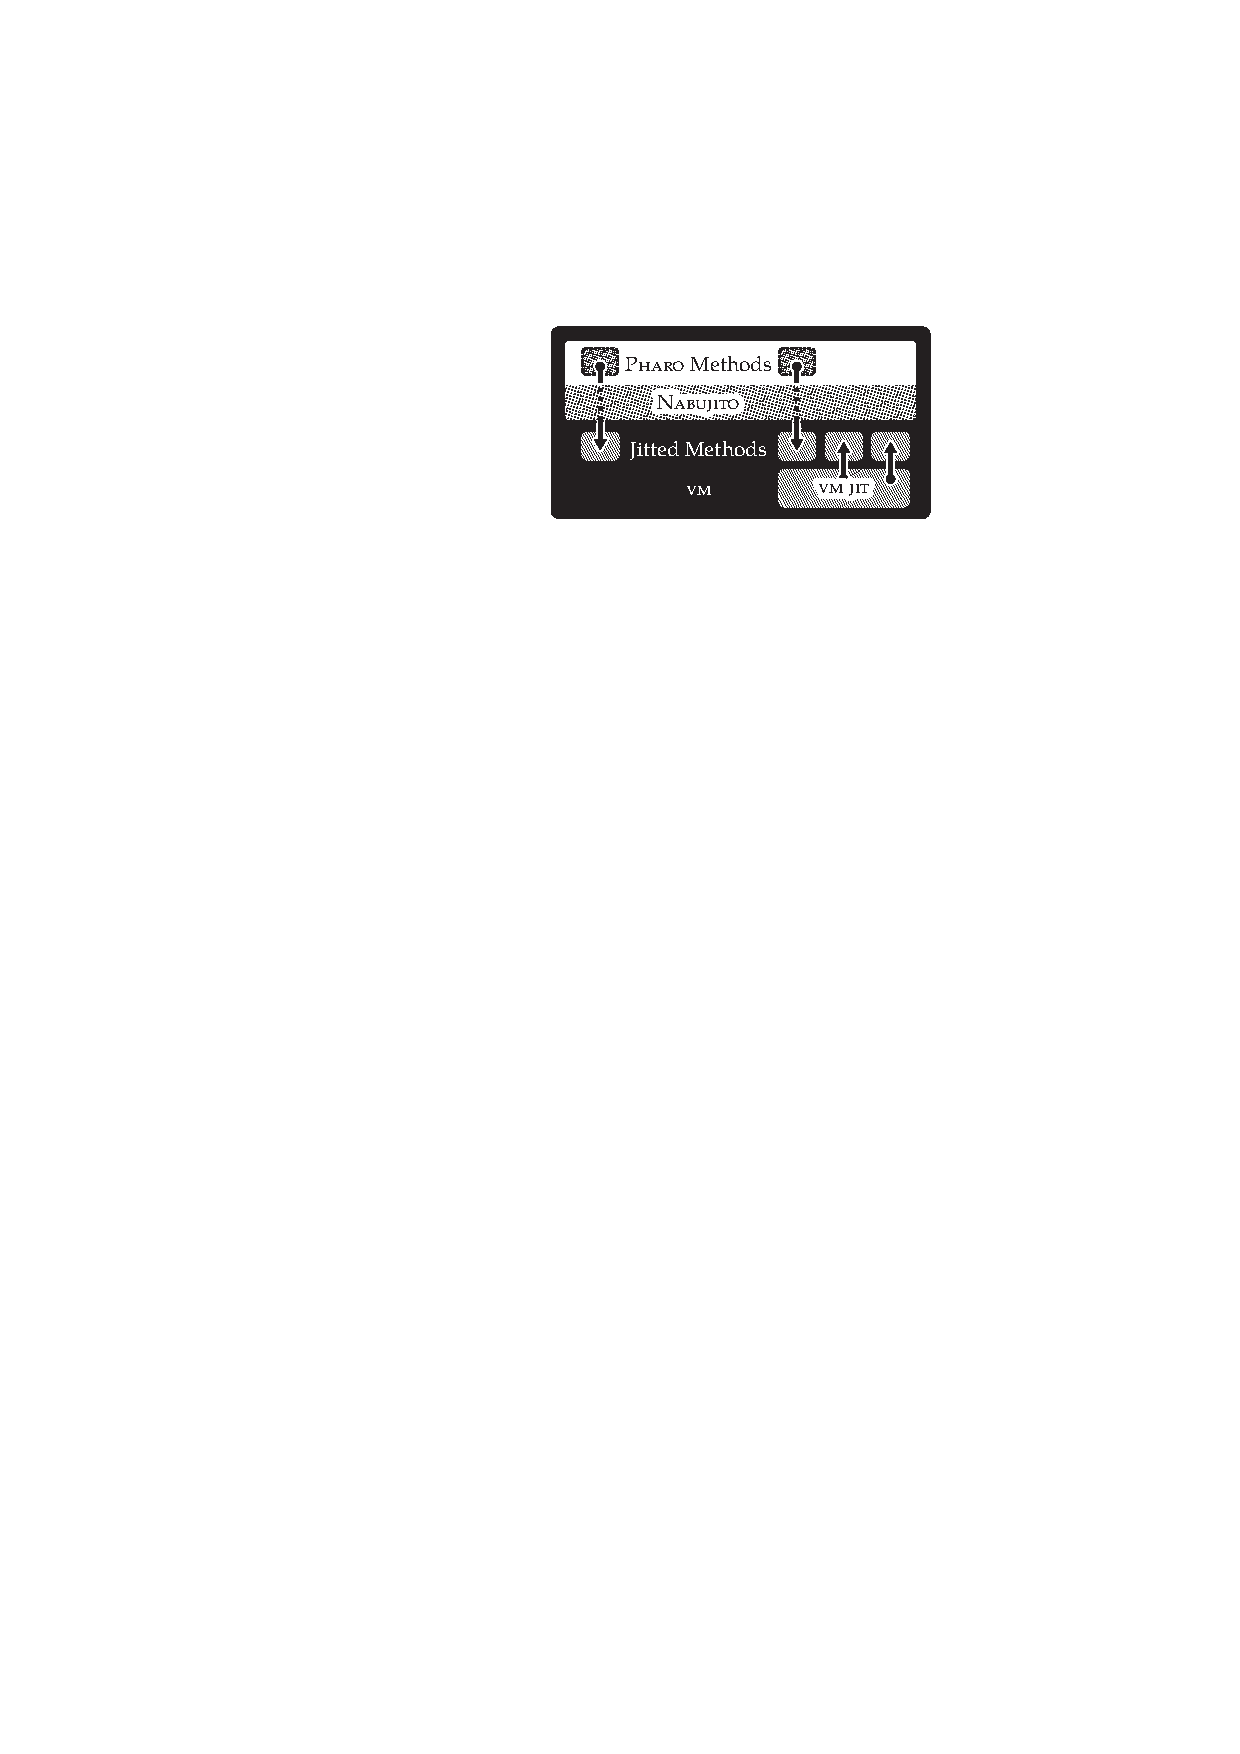
\includegraphics[scale=1.1]{nabujito-overview}
\end{figure}
\todo{Introduction}

% ---------------------------------------------------------------------------
\subsection{Background}
\seclabel{val-nabujito-background}
% ---------------------------------------------------------------------------
In this section we present \NBJ, a \B-based approach for a language-side \JIT compiler.
\NBJ goes even further than \WF using almost the same techniques.
However, instead of focusing on primitives, \NBJ generates native executable code for standard \ST methods.
Primitives tend to be more low-level, whereas \NBJ focuses on high-level \ST code. 


%----------------------------------------------------------------------------
\paragraph{The \JIT of the \PH \VM}
The \PH \VM (Cog) already comes with a \JIT that translates bytecodes to native instructions.
It transforms \ST methods into slightly optimized native code at runtime.
The main speed improvement comes from avoiding bytecode dispatching and by inlining certain known operations and primitives \cite{Ayco03a}.
The most complex logic of the \JIT infrastructure deals with the dynamic nature of the \ST environment.
Methods and classes can be changed at runtime and that has to be addressed by the \JIT infrastructure.
The \JIT compiler, by which we refer in this context to the transformation of bytecodes to native code, represents a small part of the whole infrastructure.
There exists more important stages as an additional register allocation pass to reduce the number of stack operations \cite{Mira99a,Mira11a}.
The existing \JIT infrastructure is implemented in \Slang \cite[Ch.\ 5]{Blac09a} as the rest of the \VM.

%----------------------------------------------------------------------------
\paragraph{Limitations of \VM-level \JIT Compilers}
In the context of \NBJ we separate a \JIT infrastructure into separate parts.
The major part is to have a \VM that uses stack-mapping.
In the case of a bytecode-based interpreter, we assume that the \VM provides routines to switch between a bytecode interpretation context and a low-level native execution context.
With \NBJ we move the \JIT compiler,the part that generates native code at runtime, from the \VM to the image.%, the part that generates native code at runtime, typically from bytecodes.
 Since the \JIT compiler is quite decoupled from the rest of the \JIT infrastructure we believe that a hard-coded static and low-level implementation is not optimal for several reasons:

\begin{itemize}
	\item Optimizing \ST code requires strong interactions with the dynamic environment.
	\item Accessing language-side properties from the \VM-side is hard.
	\item Changing the JIT compiler requires changes at \VM-level.
	\item The JIT reimplements primitives for optimization reasons resulting in code duplication.
\end{itemize}

\paragraph{Optimization Limitations for \PH}
In \ST methods tend to be very small and it is considered good practice to delegate behavior to other objects.
This implies that several common optimization techniques for static languages do not work well.
Dynamic method activation does not provide enough context for a static compiler to optimize methods.
Hence after inline caches and register allocation the next optimization technique is inlining.
However, inlining in a dynamic context is difficult and requires hooks at \VM-level to invalidate native code when the language-side changes.
Since in \PH, compiling a method to bytecode is handled completely with language-side code most of the infrastructure to get notified about method changes is already present.

\paragraph{Primitives in the Existing JIT}
The existing JIT reimplements the most used primitives at \VM-level.
This guarantees that the \VM stays as long as possible in the \JIT context (see \secref{benzo-jit-interaction} on page~\pageref{sec:benzo-jit-interaction}).
Additionally this enables new performance optimizations that for instance are hard to achieve with standard compliant C code.
A typical example is the integer addition which has to deal with overflow checks and conversion of tagged integers.
In \secref{val-waterfall} we describe how \WF suffers a similar constraint.
\WF manually defines such primitives in terms of native assembler instructions through the language-side \B interface.
\NBJ reuses the same optimized primitives so we rely on a single optimized definition which is shared among all native code libraries.

%----------------------------------------------------------------------------
\subsection{Implementation}
\seclabel{val-nabujito-implementation}
%----------------------------------------------------------------------------
\todo{EXTEND: Show more internals}
\todo{Add overview picture}
\NBJ is an experimental JIT implementation which replaces the bytecode to native code translation of the existing JIT infrastructure with a dynamic language-side implementation.
\NBJ is implemented mainly with a visitor strategy over the existing intermediate bytecode representation. 
Additionally we reimplemented vital native routines for the JIT which are not directly exported by the \VM using \B. 
Nabujito relies on the following \VM-level infrastructure to manage and run native code for any \PH method:

\begin{itemize}[noitemsep]
	\item Fixed native code memory segments.
	\item Routines for switching contexts.
	\item Native stack management.
\end{itemize}


\paragraph{\NBJ Compiler Steps}
\todo{Overview Figure of the input / transformation steps} \\
\todo{Almost Reified Cog Routines} \\
\todo{CogMethod patching problem leading to the following parargraph}


\paragraph{Dynamic Code Generation}
To simplify the implementation we decide to manually trigger JIT compilation.
For primitives known by \WF we rely on that infrastructure to generate the native code.
For standard methods \NBJ takes the bytecodes and transforms them to native code.
It also applies optimizations such as creating low-level branches for \ST level branching operations like \ttt{ifTrue:}.
Optimizations for additional methods are all implemented flexibly at language-side.
Wherever possible, we reimplement the same behavior as the existing native \JIT compiler.
Eventually the native code is ready and \B attaches it to the existing compiled method.
When the language-side jitted code is activated \B ensures that we do not have to leave the \JIT execution mode, and thus we can call methods at the same speed as the existing \JIT.
\todo{figure showing an extended method installation into \JIT space}


\paragraph{The \Cog \JIT}
\todo{explain the \Cog infrastructure}\\
\todo{Step 1: Native Stack Mapping as requirement}\\
\todo{Step 2: transform bytecodes to native code}\\
\todo{Step 3: Trampolines to jump back and forth between native activated scheme and bytecode interpreter based approach}\\
\todo{Step 4: Minor summary of the how the ICs work in the \JIT}

\begin{figure}
	\centering
	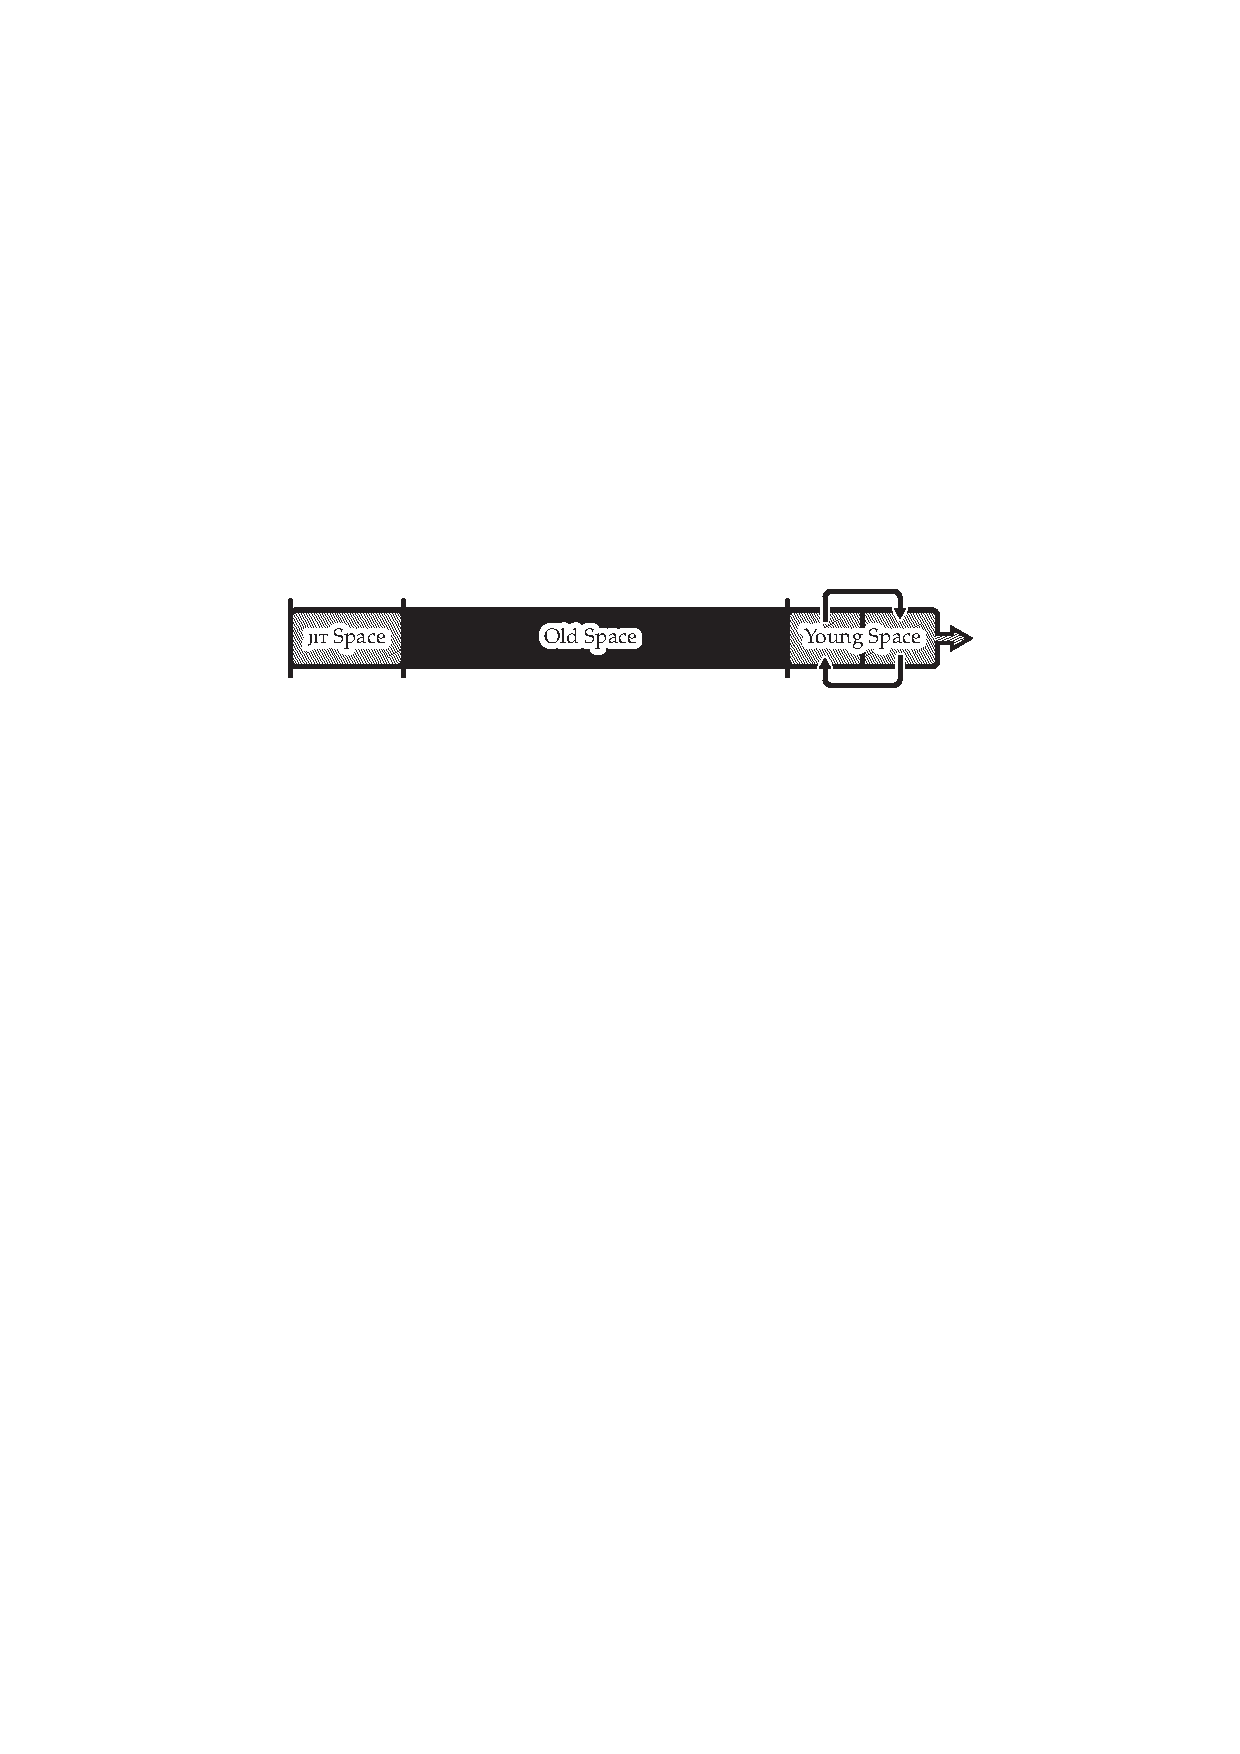
\includegraphics[scale=1.1]{cog-memory}
	\caption[\Cog Memory Model Overview]{\Cog Memory Model Overview: Fixed-sized \JIT space, slow changing old space and fast young space}
	\figlabel{[cog-memory]}
\end{figure}

\paragraph{Overcoming the Missing \VM Interface for the \JIT}
\todo{why do we need patch methods?}\\
\todo{Explain how the patch methods work}\\
\todo{give example of the assember of a simple method with the patch call}

% -----------------------------------------------------------------------------
\subsection{Validation}
\seclabel{val-nabujito-performance}
% -----------------------------------------------------------------------------

\todo{missing intro}

% -----------------------------------------------------------------------------
\subsubsection*{Compilation Time}


The performance evaluation for our \B-based \JIT compiler is focused on the language-side code-generation part.
\NBJ essentially generates the same native code as the \VM-level \JIT, hence there is no performance difference at evaluation time.
However, \NBJ is clearly slower during the warm-up phase.
Compilation of the native instructions will take considerably more time compared to the \VM-level implementation of the same bytecode to assembler transformation.
The cost of transforming the bytecodes to native code at \VM-level can be measured in native instructions, whereas the unit at language-side is bytecodes.
However, we point out again, that this is a one-time overhead.
From the in-production experience of \NB, the \B-based \FFI (see \secref{ffi-evaluation}), we know that these costs amortized, especially for long-term applications.
Instead of focusing on the final performance of the generated code, we present the compilation time compared to the normal \PH bytecode compiler, which also resides at language-side.

\begin{table}[!ht]
    \centering
    \begin{tabular}{rS}
                      & {Compilation Time [ms]} \\\midrule
        \PH Compiler  & 71(1) \\
        \NBJ          & 73(1)
    \end{tabular}
    \caption[\NBJ Compilation Speed]{Compilation efforts of the standard \ST compiler in \PH and \NBJ for the a simple method returning the constant \ttt{nil}.}
    \tablabel{val-nabujito-performance-small}
\end{table}

\noindent In \tabref{val-nabujito-performance-small} we compare the compilation speed of the standard \PH compiler and \NBJ.
We measure the accumulated time spent to compile the method 1000 times.
The average and deviation are taken over 100 runs. 
The \PH compiler takes source code as input and outputs \ST bytecodes.
\NBJ takes bytecodes as input and outputs native code.

We see that in the simple case displayed in \tabref{val-nabujito-performance-small} \NBJ's compilation speed lies within the same range as the standard \ST compiler.
We expect that in the future we apply more low-level optimizations and thus increase the compilation time of \NBJ.
However, we have shown in the performance evaluation for \NB, the \B-based \FFI, in \secref{ffi-evaluation} that even a rather high one-time overhead is quickly amortized.
Furthermore with \ST's image approach the generated native code is persistent over several sessions.
A subsequent restart of the same runtime will not cause the \JIT to nativize the same methods it did during the last launch.
Hence our approach is even valid for short-timed script-like applications as most of the methods will already be available in optimized native code from a previous run.

% -----------------------------------------------------------------------------
\subsubsection*{Per Method Comparison}
\todo{choose simple enough methods that we can compile with nabujito: currently only + works}


% -----------------------------------------------------------------------------
\subsection{Problems}
\seclabel{val-nabujito-problems}
% -----------------------------------------------------------------------------
\paragraph{Hidden \VM Internals}
\todo{backref to patch methods}\\
\todo{maintenance problem: \NBJ harcodes the \VM interaction}


\paragraph{Debugging Cycle}
\todo{Missing tools to directly interact with benzo / the real vm} \\
\todo{missing small assembler tests} \\
\todo{reactivate the VM simulator infrastructure}

\paragraph{Missing Optimizations}
One major performance optimization missing in both, the original \PH \VM-level \JIT and \NBJ, is inlining. 
By inlining we are able to create methods that are potentially big enough for optimizations.
However, inlining is a difficult task in a highly dynamic language such as \ST or \Self \cite{Cham89a}. 
Efficient inlining can only be performed with sufficient knowledge of the system. 
Accessing this high-level information from within the \VM is cumbersome and requires duplication of language-side reflective features.
The \JIT lives on the same level as the information it needs relying on the already present reflective features of \ST.


% ===========================================================================
\section{Outlook}
% ===========================================================================

\todo{Common problem: missing debugging infrastructure} \\
\todo{\WF and \NBJ share the same problems} \\
\todo{For speed a proper \JIT interface is missing } \\


% ===========================================================================
\section{Summary}
% ===========================================================================


% =============================================================================
\ifx\wholebook\relax\else
    \end{document}
\fi